\subsection{Moorovy grafy}


Motivací nechť jsou r-regulární grafy bez krátkých cyklů (troj- a 
čtyřúhelníků). Triviální konstrukce nám dává odhad na počet vrcholů:
\begin{align}
\label{moorova-podminka}
	|V| \geq 1 + r + r(r-1) = r^2 +1
\end{align}

\begin{center}
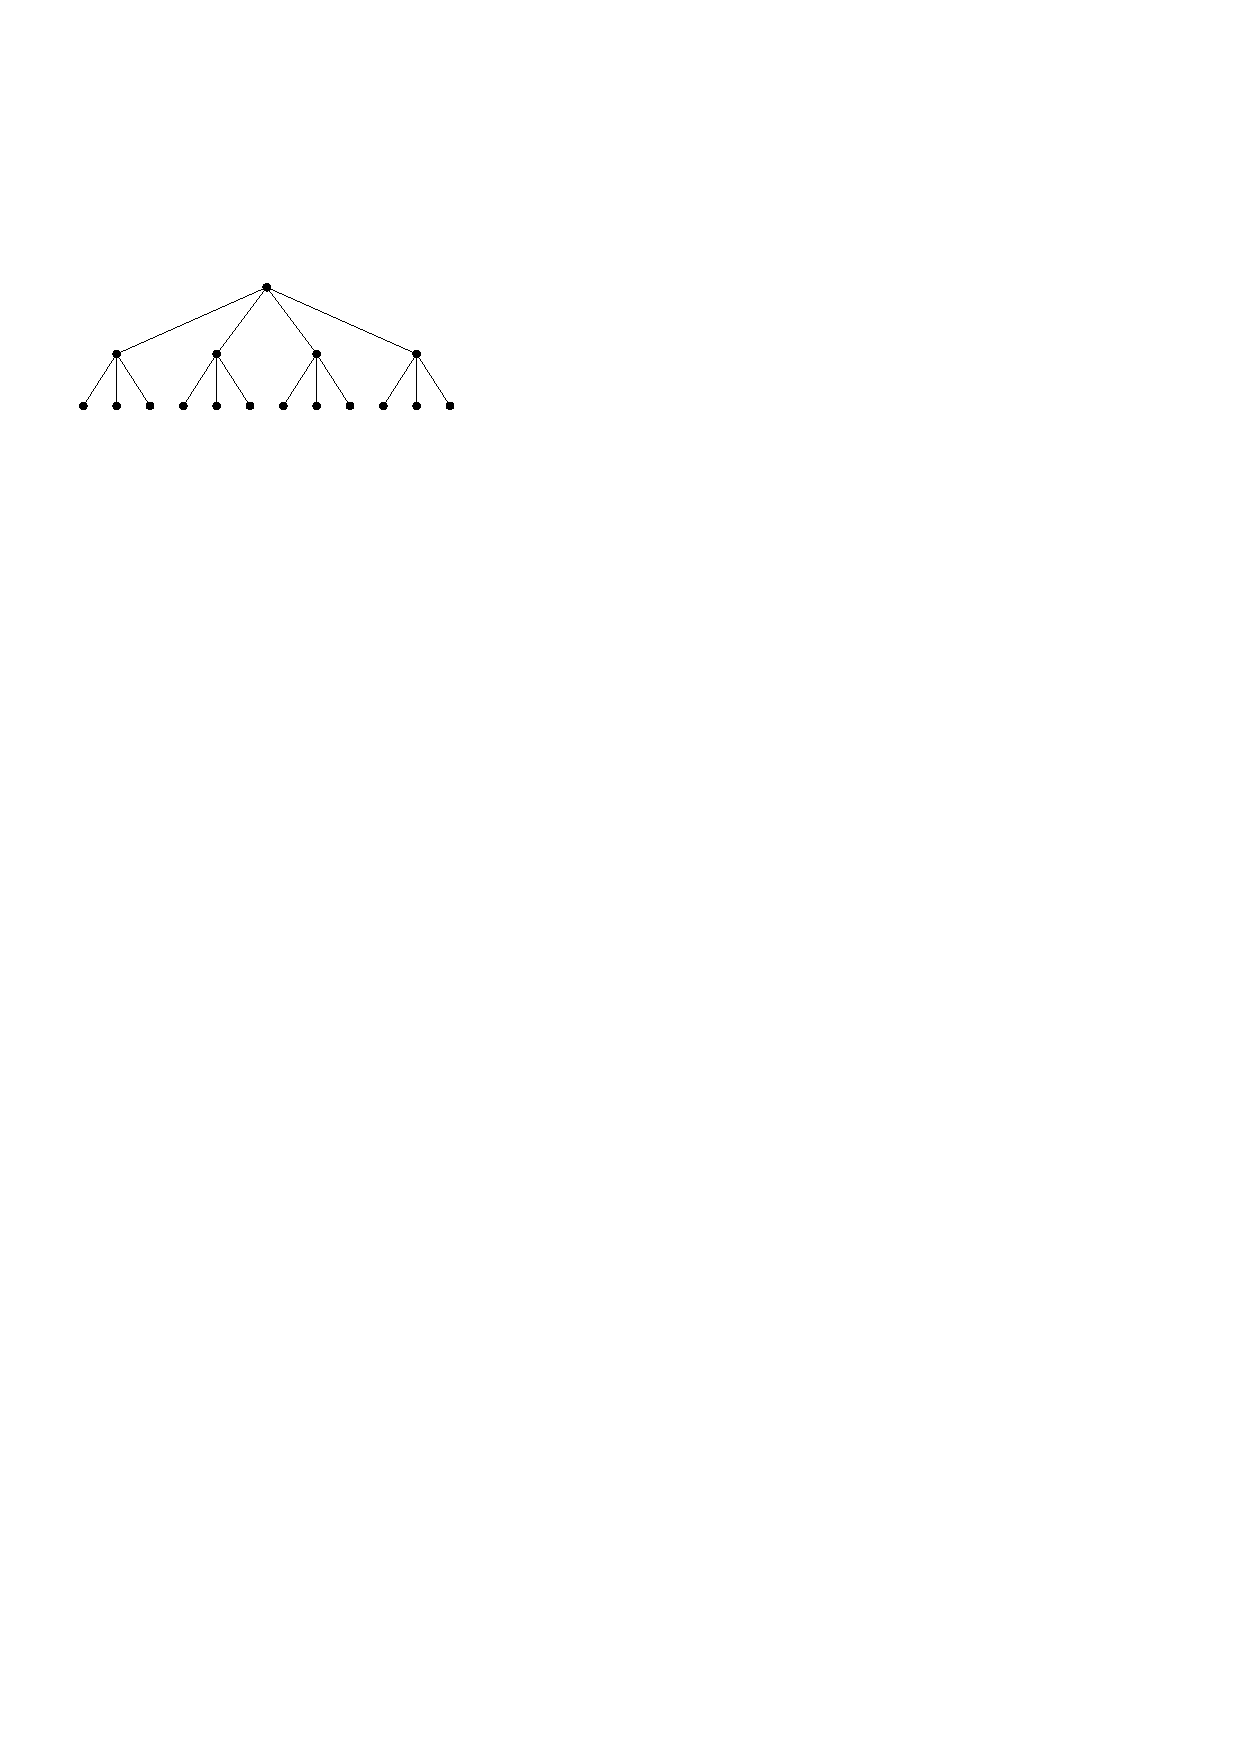
\includegraphics{moore.pdf}
\end{center}

\df Moorův graf je takový $r$-regulární graf bez troj- a čtyř-úhelníků, kde 
platí v (\ref{moorova-podminka}) rovnost.

\vt Moorův graf existuje pro $r=1,2,3,7$, pro $r=57$ se neví a pro žádné další 
$r$ neexistuje.

\dk (Idea) Mějme graf $G$ Moorův a $A$ jeho matici sousednosti. Zapišme druhou 
mocninu $A$ jako stupeň na diagonále a prohozené 0 a 1 jinde a upravme:
\begin{align}
	&A^2 = rE + {\bf0} + {\bf1}(J- A-E) \\
	&A^2 = rE - J - A - E \\
	\label{moorova-matice}&A^2 + A + (1-r)E = J
\end{align}
Dále pro nějaké $\lambda\in \Sp(A)$:
\begin{align}
	\label{moorova-mocnina}A^2 x = AAx = A\lambda x = \lambda A x = \lambda 
	\lambda x = \lambda^2 x
\end{align}
A dosadíme (\ref{moorova-matice}) za $A$:
\begin{align}
	Jx = (A^2 + A + (1-r)E)x = (\lambda^2 + \lambda + (1-r))x
\end{align}
A tedy $(\lambda^2 + \lambda + 1 -r) \in \Sp(J)$. Vlastní čísla matice $J$ 
(matice samých jedniček) ale známe, jsou to $\{0^{(n-1)}, n^{(1)}\}$. Zjevně pro 
$\lambda = r$ vyjde vlastní číslo $n$, je tedy potřeba vyřešit kvadratickou 
rovnici s parametrem $r$:
\begin{align}
	\lambda^2 + \lambda + 1 - r = 0
\end{align}
Jak na to půjdeme? Vyjádříme si $\lambda$ známým vzorečkem pro kořeny:
\begin{align}
	\lambda_{1,2} = \frac{-1\pm \sqrt{1-4(1-r)}}{2} = \frac{-1\pm\sqrt{4r-3}}{2}
\end{align}
Násobnost označíme $m_1, m_2$. Protože stopa matice je suma vlastních čísel 
včetně násobností, platí dále rovnice (protože matice sousednosti $A$ má na 
diagonále vždy nuly):
\begin{align}
	\Tr(A) = r+m_1\lambda_1 + m_2\lambda_2 = 0
\end{align}
Nejdříve
upravíme do formy (násobení dvěma a přeskupení):
\begin{align}
	2r - r^2 + \sqrt{4r-3}(m_1 - m_2) = 0 \label{4-2:rovnice}
\end{align}
Všimneme si, že $r\in\N$, tedy máme dvě možnosti:
\begin{enumerate}
	\item $\sqrt{4r-3} \not\in \Q$: potom $m_1 = m_2$ a tedy $r = 2$.
	\item $\sqrt{4r-3} = s \in \Q$, což implikuje\footnote{Odmocnina z celého čísla je
  vždy celé číslo či iracionální číslo, nikdy zlomek.} $s \in \N$.
  Substitucí $4r - 3 = s^2$ do rovnice \ref{4-2:rovnice} získáme
	$s \in \set{1, 3, 5, 15}$, což dává $r \in \set{1, 3, 7, 57}$.
\end{enumerate}
\qed


